%Text Books : \cite{balakrishnan}
%Module I:
%Introduction, Basic concepts. Sub graphs. Degrees of vertices. Paths and Connectedness, Automorphism of a simple graph, line graphs, Operations on graphs, Graph Products.
%Directed Graphs : Introduction, basic concepts and tournaments.
%(Chapter 1 Sections 1.1 – 1.7( Upto 1.7.3 including ) 1.8, 1.9)
%(Chapter 1 Sections 2.1, 2.2, 2.3) (20Hours)
%Module II:
%Connectivity : Introduction, Vertex cuts and edge cuts, connectivity and edge connectivity, blocks, Cyclical edge Connectivity of a graph.
%Trees; Introduction, Definition, characterization and simple properties, centres and cancroids, counting the number of spanning trees, Cayley’s formula.
%Applications
%(Chapter 3 Sections 3.1, 3.2 , 3.3, 3.4 and 3.5 )
%(Chapter 4 Sections4.1, 4.2, 4.3, 4.4 (Up to 4.4.3 including ) and 4.5, 4.7) (25Hours)
%Module III:
%Eulerian and Hamiltonian Graphs: Introduction, Eulereian graphs,
%Hamiltonian Graphs, Hamiltonian around’ the world’ game
%Graph Colorings: Introduction, Vertex Colorings, Applications of Graph Coloring, Critical Graphs, Brooks’ Theorem
%(Chapter 6 Sections 6.1, 6.2 and 6.3 )
%(Chapter 7 Sections 7.1, 7.2 and7.3(Up to 7.3.1 including ) (20Hours)
%Module IV:
%Planarity: Introduction, Planar and Nonplanar Graphs, Euler Formula and Its Consequences, K5 and K 3,3 are Nonplanar Graphs, Dual of a Plane Graph, The Four-Color Theorem and the Heawood Five-Color Theorem .
%Spectral Properties of Graphs: Introduction, The Spectrum of a Graph, Spectrum of the Complete Graph Kn, Spectrum of the Cycle Cn,
%(Chapter 8 Sections 8.1, 8.2 , 8.3, 8.4, 8.5 and 8.6 )
%(Chapter 11 Sections 11.1, 11.2 , 11.3 and 11.4) (25Hours)

%Module 1 - \cite{balakrishnan} 1, 2
%Module 2 - \cite{balakrishnan} 3, 4
%Module 3 - \cite{balakrishnan} 6, 7
%Module 4 - \cite{balakrishnan} 8, 11
%Missing - \cite{balakrishnan} 5, 9, 10, ?

%\chapter{Basic Results}
\section{Basic Results}
\subsection{Introduction}
\cite{balakrishnan}
\subsection{Basic Concepts}
\begin{definition}
	A \textbf{graph} is an ordered triple $G = (V,E,I)$ where $V$ is a nonempty set of vertices, $E$ is a set of edges and $I$ is an incidence map which associates each edge with an unordered pair of vertices.
\end{definition}

\begin{description}
	\item[end vertices] Let $e$ be an edge with $I_G(e) = \{ u,v \}$. Then $u,v$ are the end vertices of $e$. We may write $e = uv$.
	\item[incident] An edge $e =uv $ said to be incident on both vertices $u$ and $v$. Then vertices $u$ and $v$ are incident on edge $e$ as well. 
	\item[parallel edges] are those edges which have same pair of end vertices.
	\item[loop] is an edge whose both end vertices are the same.
	\item[neighbour] Vertex $u$ is neighbour of vertex $v$ if $uv$ is an edge of the graph.
	\item[Open neighbourhood] $N(u)$ is the set of all neighbours of the vertex $u$.
	\item[Closed neighbourhood] $N[u] = N(u) \cup \{ u \}$.
	\item[simple] graph does not have any parallel edges or loops.
	\item[adjacent] Two vertices $u,v$ are adjacent if both $u,v$ are incident on an edge, say $uv$. Two edges are adjacent if they have a common end vertex.
\end{description}
\begin{definition}
	A graph is \textbf{finite} if both vertex set $V$ and edge set $E$ are finite. A finite graph, $G$ order, $n(G) = |V(G)|$ and size, $m(G) = |E(G)|$. Or simply $n = |V(G)|$ and $m = |E(G)|$.
\end{definition}

\begin{definition}
	A graph $G$ is \textbf{labeled} if its vertices are distinguished from one another by means of distinct labels.
\end{definition}

\begin{definition}
	Two graphs $G$ and $H$ are \textbf{isomorphic} if there exists a pair $(\phi,\theta)$ where $\phi : V(G) \to V(H)$ and $\theta : E(G) \to E(H)$ are bijections such that $I_G(e) = \{ u,v \} \iff I_H(\theta(e)) = \{ \phi(u),\phi(v) \}$.\\

	Two simple graphs $G$ and $H$ are \textbf{isomorphic} if there exists a bijection $\phi : V(G) \to V(H)$ which induced another bijection $\theta : E(G) \to E(H)$ such that $I_G(e) = \{ u,v \} \iff I_H(\theta(e)) = \{ \phi(u),\phi(v) \}$.
\end{definition}

\begin{exercise}
	Let $G$, $H$ be simple graph and let $\phi : V(G) \to V(H)$ be a bijection such that $uv \in E(G) \implies \phi(u)\phi(v) \in E(H)$. Show that $\phi$ is not an isomorphism.
\end{exercise}
	Let $G,H$ be simple graph with bijection $\phi : V(G) \to V(H)$.
	If there exists two vertices $u,v$ which are non-adjacent in $G$, but $\phi(u),\phi(v)$ are adjacent in $H$.
	Then $\phi$ is not an isomorphism.

\begin{definition}
	A simple graph is \textbf{complete} if every pair of distinct vertices are adjacent.
	A complete graph with $n$ vertices is denoted by $K_n$.
	Then $m(K_n) = \binom{n}{2} = \frac{n(n-1)}{2}$.
	A \textbf{totally} disconnected graph has no edges.
	Thus, $0 \le m \le \binom{n}{2}$.
	A graph $G$ is trivial if it has only one vetex and no edges.
\end{definition}

\begin{definition}
	A graph $G$ is \textbf{bipartite} if its vertex set can be partitioned into two nonempty sets $X$ and $Y$ such that every end of $G$ has one end in $X$ and the other end in $Y$. We write $G(X,Y)$ is bipartite with partition $X,Y$.
	A simple, bipartite graph $G(X,Y)$ is \textbf{complete bipartite} if every vertex in $X$ is adjacent to every vertex in $Y$. Let $G(X,Y)$ be a complete bipartite graph with $|X| = p$ and $|Y|=q$, then we write $K_{p,q}$. A graph of the form $K_{1,q}$ is called a \textbf{star}.
\end{definition}

\begin{remark}
	Let $G$ be a complete bipartite graph, $K_{p,q}$.
	Then it has order $n = p+q$ and size $m = pq$.
\end{remark}

\begin{definition}
Let $G$ be a graph. The complement $G^c$ of graph $G$ is the graph with same vertex set. Two vertices $u,v$ of $G^c$ are adjacent if and only if $u,v$ are non-adjacent in $G$.
	$$ V(G^c) = V(G) \quad \& \quad uv \in E(G^c) \iff uv \notin E(G) $$
\end{definition}
\begin{remark}
	We have, $(G^c)^c = G$, since ${uv \in G \iff uv \notin G^c \iff uv \in (G^c)^c}$ and $V(G) = V(G^c) = V((G^c)^c)$.
	Let $G$ be a graph of order $n$, then $E(G) + E(G^c) = E(K_n)$ as each edge of $K_n$ is either an edge of $G$ or an edge of $G^c$.
\end{remark}

\begin{definition}
	A simple graph is self-complementary if $G \cong G^c$.
\end{definition}
\begin{remark}
	The order of a self complementary graph $G$ of order $n$ is $n(n-1)/4$ since $m(G) = m(G^c)$ and $m(G) + m(G^c) = m(K_n)$.
\end{remark}

\subsection{Subgraphs}
\begin{description}
	\item[subgraph] A graph $H$ is a subgraph of $G$ if $V(H) \subset V(G)$, $E(H) \subset E(G)$ and $I_H$ is $I_G$ restricted to $E(H)$. Then $G$ is a \textbf{supergraph} of $H$.
	\item[induced subgraph] Let $G$ be a graph and $S$ be a subset of the vertex set of $G$. The subgraph induced by $S$, $G[S]$ has vertex set $S$ and two vertices are adjacent only if they are adjacent in $G$.
	\item[edge induced subgraph] Let $G$ be a graph and $S$ be a subset of the edge set of $G$. The subgraph induced by the edge set $S$ is denoted by $G[S]$. Vertex $u$ is a vertex of $G[S]$ only if $S$ has an edge incident on it.
	\item[spanning subgraph] Let $H$ be a subgraph of graph $G$. If $V(H) = V(G)$, then $H$ is a spanning subgraph.
	\item[clique] is a subgraph which is complete. A clique is maximal if it is not contained in another clique.
\end{description}

\begin{remark}
	If an edge $e$ is deleted from a graph $G$, then vertex set remains the same. The graph $G-\{e\}$ is a spanning subgraph of $G$.
	If a vertex $u$ is deleted from a graph $G$, then all the edge incident on $u$ are also deleted. The graph $G-\{u\}$ is an induced subgraph of $G$.
\end{remark}

\subsection{Degree of Vertices}
\begin{definition}
	Let $G$ be a graph and $u$ be a vertex of $G$.
	The \textbf{degree} of $u$ is the number of edges incident on it with multiplicities. That is, every loop incident on $u$ is counted twice.
\end{definition}
\begin{remark}
	In a simple graph, the degree of a vertex is the cardinality of its open neighbourhood.
	$\deg_G(u) = |N_G(u)|$.
\end{remark}

\begin{definition}
	A graph $G$ is $k$-\textbf{regular} if every vertex is of degree $k$. Graph $G$ is \textbf{regular} if it is $k$-regular for some $k$. \textbf{Cubic} graphs are the $3$-regular graphs.
\end{definition}
\begin{remark}
	Complete graph $K_{n+1}$ are $n$-regular.
	And complete graphs are the smallest regular graphs.
	$K_4$ is cubic.
	Petersen graph is cubic.
\end{remark}
\begin{figure}
\centering
\scalebox{0.9}{
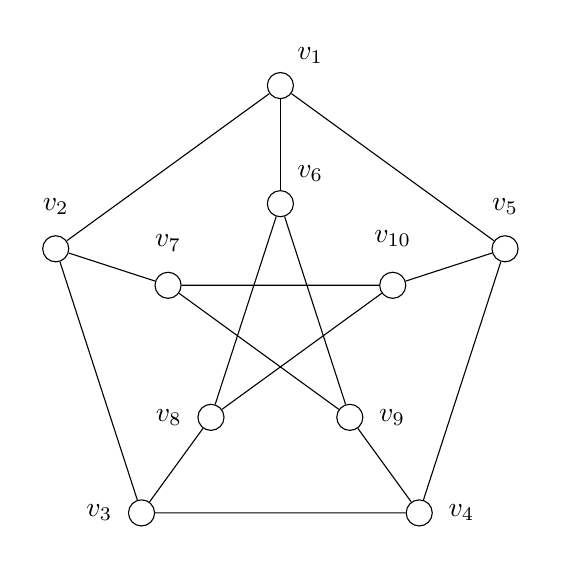
\begin{tikzpicture}
	\node (u){};
	\tikzstyle every node=[draw,circle]
	\draw (u) ++(90:1.5) node (b1)[label=above right:$v_6$]{};
	\draw (u) ++(162:1.5) node (b2)[label=above:$v_7$]{};
	\draw (u) ++(234:1.5) node (b3)[label=left:$v_8$]{};
	\draw (u) ++(306:1.5) node (b4)[label=right:$v_9$]{};
	\draw (u) ++(18:1.5) node (b5)[label=above:$v_{10}$]{};

	\draw (u) ++(90:3) node (a1)[label=above right:$v_1$]{};
	\draw (u) ++(162:3) node (a2)[label=above:$v_2$]{};
	\draw (u) ++(234:3) node (a3)[label=left:$v_3$]{};
	\draw (u) ++(306:3) node (a4)[label=right:$v_4$]{};
	\draw (u) ++(18:3) node (a5)[label=above:$v_5$]{};

	\draw (b1)--(b3)--(b5)--(b2)--(b4)--(b1);
	\draw (a1)--(a2)--(a3)--(a4)--(a5)--(a1);

	\draw (a1)--(b1);
	\draw (a2)--(b2);
	\draw (a3)--(b3);
	\draw (a4)--(b4);
	\draw (a5)--(b5);
\end{tikzpicture}
}
\end{figure}
\begin{remark}
	The complement of a regular graph is also regular. If $G$ is $k$-regular, then $G^c$ is $r$-regular where $k+r = n-1$.
\end{remark}
\begin{description}
	\item[1-factor] is a spanning, $1$-regular subgraph.
	\item[isolated vertex] is a vertex with degree $0$.
	\item[pendent vertex] is a vertex with degree $1$.
	\item[pendent edge] is the only edge incident on a pendent vertex.
\end{description}

\begin{theorem}[Euler]
	The degree sum of a graph is twice its size.
\end{theorem}
\begin{proof}
	Every edge $e= uv$ contributes $1$ to the degree of both the end vertices $u$ and $v$. Thus every edge contributes $2$ to the degree sum. There are $m$ edges, thus degree sum is $2m$.
\end{proof}

\begin{corollary}
	In a grpah $G$, the number of vertices of odd degree is even.
\end{corollary}
\begin{proof}
	Let $G$ be a graph of order $n$.
	Let $V_1,V_2$ be the set of vertices of even,odd degree respectively.
	Then, $\sum d_i = \sum_{v \in V_1} \deg(v) + \sum_{v \in V_2} \deg(v)$.
	The degree sum is even and the first sum on RHS is also even. Thus the second sum should be even. Since, each term in the second sum is an odd integer, there are even number of terms in the second sum. In other words, there are even number of vertices with an odd degree.
\end{proof}
\begin{exercise} 
	If $G \overset{\phi}{\cong} H$, then each pair $u,\phi(u)$ have the same degree.
\end{exercise}
Let $G,H$ be isomorphic graphs.
Let $u$ be a vertex of $G$.
A vertex $v$ is adjacent of $u$ in $G$ if and only if $\phi(v)$ is adjacent to $\phi(u)$ in $H$. Thus, $\deg_G(u) = \deg_H(\phi(u))$.

\begin{remark}
	Clearly, a graph isomorphism preserves adjacency, degree of vertices and neighbourhoods, etc.
	$N_H(\phi(u)) = \{ \phi(v) : v \in N_G(u) \}$.
\end{remark}

\begin{exercise}
	Let $d : d_1,d_2,\dots,d_n$ be the degree sequence of a graph $G$.
	Let $r$ be a positive integer, then $\sum d_i^r$ is even.
\end{exercise}
Let $G$ be a graph of order $n$.
Let $V_1,V_2$ be the set of vertices of even and odd degree respectively.
Clearly, $\sum d_i^r = \sum_{v \in V_1} d_i^r + \sum_{v \in V_2} d_i^r$.
Once again, the first sum on RHS is even as $d_i^r$ is even when $d_i$ is even. And the second sum is odd as $d_i^r$ is odd when $d_i$ is odd. By Euler`s theorem, there are an even number of such odd terms. Thus, the second sum on RHS is also even. Therefore, $\sum d_i^r$ is even.

\begin{definition}
	A sequence of nonnegative integers $d : d_1,d_2,\dots,d_n$ is \textbf{graphical} if there exists a \textit{simple} graph with degree sequence $d$.
\end{definition}

\begin{example}
	The sequence $d : 7,6,3,3,2,1,1,1$ is nongraphical. Let $v_0,v_1$ be the vertics with degree $7,6$ respectively. Then for $d$ to be graphical, there should be at least another $4$ vertices with degree greater than or equal to $2$.
	This is not the case, therefore $d$ is not graphical.
\end{example}

\begin{exercise}
	Let $d : d_1,d_2,\dots,d_n$ is a sequence of nonnegative integers with $\sum d_i$ even. Show that there exists a non-simple graph with $d$ as its degree sequence.
\end{exercise}
	Let $d : d_1,d_2,\dots,d_n$ be a sequence of nonnegative integers with $\sum d_i$ even. Then there are even number of odd integers (if any).\\

	Step 1 : Draw a vertex $u_i$ for each term $d_i$.
	If a pair $(d_i,d_j)$ is odd\footnote{If you want maximal simple graph, you may add an edge $u_iu_j$(if it not already there) and subtract $1$ from both $d_i$ and $d_j$, provided both $d_i$ and $d_j$ are nonzero.}, then draw an edge $u_iu_j$ and subtract $1$ from both $d_i$ and $d_j$.\\

	Step 2 : If $d_i = 2k$. Draw $k$ loops on $u_i$.\\

\begin{challenge}
	Draw maximal connected graph for a degree sequence ?
\end{challenge}

\begin{application}
	In any group of $n$ persons ($n \ge 2$), there are at least two with same number of friends.
\end{application}
\begin{proof}
	Suppose group of $n$ persons is modelled by a graph with $n$ vertices and two vertices are adjacent if the respective persons are friends. It is assumed that friendship is mutual, otherwise it is not considered. Suppose all of them have different number of friends. Then every vertex in the graph has different degree.\\

	The possible degree of a vertex in a graph of order $n$ is $0,1,\dots,(n-1)$. Since all $n$ vertices have different degree and we have only $n$ options. There exists a vertex of degree $j$ for each $0 \le j < n$. This leads to a contradiction.\\

	Let $v_1,v_n$ be the vertices with degree $0,(n-1)$. Then $v_n$ is adjacent to every other vertex and $v_1$ is non-adjacent to every other vertex which is not possible. Thus, at least two vertices should have same degree. Therefore, in a group of $n$ persons, at least two of them have same number of friends.
\end{proof}

\begin{exercise}
	Let $G$ be a graph in which every vertex is of degree $k$ or $k+1$. Then the number of vertices with degree $k$ is $(k+1)n-2m$.
\end{exercise}
\begin{proof}
	Let $G$ be a graph of order $n$ and size $m$.
	Let $x$ be the number of vertices with degree $k$.
	Then there are $n-x$ vertices with degree $k+1$.
	By Euler`s theorem, $ xk + (n-x)(k+1) = 2m \implies x = (k+1)n-2m$.
\end{proof}
	
\subsection{Paths and Connectedness}
\begin{definition}
	Let $G$ be a graph. A \textbf{walk} on $G$ is an alternating finite sequence of vertices and edges which starts and ends at some vertices, say $W : v_0 e_0 v_1 e_1 \dots e_k v_k$.
	The vertex $v_0$ is the \textbf{origin} and $v_k$ is the \textbf{terminus} of the walk $W$.
\end{definition}
\begin{description}
	\item[closed walk] A walk is \textbf{closed} if its origin and terminus are identical. Otherwise the walk is \textbf{open}.
	\item[trail] is a walk in which edges are distinct.
	\item[path] is a trail in which vertices are distinct.
	\item[cycle] is a closed trail in which vertices are distinct.
\end{description}

\begin{remark}
	A walk of length zero is a single vertex. And this walk is called a \textbf{trivial path}.
	Let $P : v_0,e_1,v_1,e_2,v_2,\dots,v_{k-1},e_k,v_k$ be a path in $G$. Then the \textbf{inverse of the path} is given by, $P^{-1} : v_k,e_k,v_{k-1},\dots,v_1,e_1,v_0$.
	And $v_j,e_j,v_{j+1},\dots,v_{k-1},e_{k-1},v_k$ is the $v_j-v_k$ \textbf{section} of the path $P$.
\end{remark}

\begin{definition}
	Let $G$ be a graph. Then connectedness is an equivalence relation on $V(G)$. Let $V_1,V_2,\dots,V_\omega$ be the equivalence classes. Then the induced subgraphs $G[V_1], G[V_2], \dots, G[V_\omega]$ are the \textbf{components} of $G$.
\end{definition}

\begin{remark}
	For a connected graph, $\omega = 1$. And for disconnected graphs $\omega \ge 2$. And components are maximal connected subgraphs of $G$. The number of components of $G$ is denoted by $\omega(G)$.
\end{remark}

\begin{definition}
	Let $d : V(G) \to V(G),\ d(u,v)$ is the length of the shortest $u-v$ path. If there is no $u-v$ path, then $d(u,v) = \infty$.
\end{definition}
\begin{exercise}
	Let $G$ be a simple graph.
	The vertex set $V(G)$ together with distance function $d(u,v)$, length of shortest $u-v$ path is a metric space.
\end{exercise}
\begin{proof}
	Let $G$ be a simple graph with vertex set $V(G)$ and $d : V(G) \to V(G),\ d(u,v)$ is the length of a shortest $u-v$ path.
\begin{enumerate}
	\item Every path has non-negative length. Thus, $\forall u,v \in V(G),\ d(u,v) \ge 0$.\\
	And $d(u,u) = 0$ since trivial path has zero length.
	\item Suppose $u,v$ are connected in $G$. Otherwise $d(u,v) = d(v,u) = \infty$.\\
	Let $P$ be a shortest $u-v$ path. Then $P^{-1}$ is a shortest $v-u$ path.
	Suppose there exists a $v-u$ path, $Q$ which is shorter than $P^{-1}$. Then $Q^{-1}$ is shorter than $P$ which is a contradiction.
	Thus, $d(u,v) = d(v,u)$.
	\item Suppose $d(u,v) < \infty$. Otherwise the result is trivial.\\
	Let $P,Q$ be shortest $u-w$ path, $w-v$ path in $G$. Then $P+Q$ is a $u-v$ walk.
	Thus, there exists a $u-v$ path\footnote{Every $u-v$ walk, contains a $u-v$ path which can be obtained by subsequently replacing each $w-w$ section of the walk with $w$.} of length less than or equal to the length of $P+Q$.
	Therefore, $d(u,v) \le d(u,w) + d(w,v)$.
\end{enumerate}
\end{proof}

\begin{proposition}
	If $G$ is a simple graph with $\delta(G) \ge \frac{n-1}{2}$, then $G$ is connected.
\end{proposition}
\begin{proof}
	Let $G$ be a graph of order $n$.
	Suppose $G$ is not connected. Then $G$ has at least two components, say $G_1$ and $G_2$.
	Let $v \in V(G_1)$. Since $\deg(v) \ge \frac{n-1}{2}$, there are at least $\frac{n-1}{2}$ other vertices in $G_1$.
	Thus, each component of $G$ has at least $\frac{n+1}{2}$ vertices.
	And $G$ has at least $\frac{n+1}{2} + \frac{n+1}{2}$ vertices which is a contradiction.
	Therefore, $G$ is connected.
\end{proof}

\begin{exercise}
	A simple graph with $\delta(G) \ge \frac{n-2}{2}$ is not necessarily connected.
\end{exercise}
\begin{proof}
	Let $G$ be a simple graph with $\delta(G) = \frac{n-2}{2}$ where $n$ is even. Then $G$ is not necessarily connected. For example, $2K_2$ has $\delta = 1$ and is disconnected.
\end{proof}

\begin{exercise}
	In a group of six people, there must be three people who are mutually acquainted or three people who are mutually nonacquainted.
\end{exercise}
\begin{proof}
	Suppose the result is not true.
	Then every person $u$ has at least one friend. Suppose $u$ has no friends. Then $(v,w,x)$ are mutual friends. Otherwise, either $(u,v,w)$, $(u,v,x)$ or $(u,w,x)$ are mutually non-acquainted.\\
	
\begin{figure}[hbt]
\centering
\scalebox{0.9}{
\begin{tikzpicture}
	\tikzstyle every node=[draw,circle]
	\node (u)[label=above:$u$]{};
	\node (v)[above right=1cm of u,label=above:$v$]{};
	\node (w)[below right=1cm of u,label=below:$w$]{};
	\node (x)[right=1cm of v,label=above:$x$]{};
	\node (y)[right=1cm of w,label=below:$y$]{};
	\node (z)[below right=1cm of x,label=above:$z$]{};
	\draw[dotted] (w)--(u)--(v);
	\draw[dotted] (x)--(u)--(y);
	\draw[dotted] (u)--(z);
	\draw[dashed,red] (v)--(w)--(z)--(v);
\end{tikzpicture}
}
\caption{Minimum Degree $\delta(G) > 0$}
\end{figure}
	There exists a person $u$ with at least two friends. Suppose every person has exactly one friend, say $(u,v), (w,x), (y,z)$ are friends. Then $(u,w,y)$ are mutually non-acquainted.\\

\begin{figure}[hbt]
\centering
\scalebox{0.9}{
\begin{tikzpicture}
	\tikzstyle every node=[draw,circle]
	\node (u)[label=above:$u$]{};
	\node (v)[above right=1cm of u,label=above:$v$]{};
	\node (w)[below right=1cm of u,label=below:$w$]{};
	\node (x)[right=1cm of v,label=above:$x$]{};
	\node (y)[right=1cm of w,label=below:$y$]{};
	\node (z)[below right=1cm of x,label=above:$z$]{};
	\draw (u)--(v);
	\draw (w)--(x);
	\draw (y)--(z);
	\draw[dotted,red] (u)--(w)--(y)--(u);
\end{tikzpicture}
}
\caption{Maximum degree $\Delta(G) > 1$}
\end{figure}
	Suppose $u$ has at least two friends, say $v,w$. Then $v,w$ are not friends, otherwise $(u,v,w)$ are mutual friends.
	Every other person $x,y$ and $z$ is friend of either $v$ or $w$. Suppose $x$ is not a friend of both $v$ and $w$. Then $(v,w,x)$ are mutually non-acquainted. Suppose $x$ is a friend of $v$ or $w$ or both. Then $u$ is not a friend of $x$. Otherwise either $(u,v,x)$ or $(u,w,x)$ are mutual friends.\\

\begin{figure}[hbt]
\centering
\scalebox{0.9}{
\begin{tikzpicture}
	\tikzstyle every node=[draw,circle]
	\node (u)[label=above:$u$]{};
	\node (v)[above right=1cm of u,label=above:$v$]{};
	\node (w)[below right=1cm of u,label=below:$w$]{};
	\node (x)[right=1cm of v,label=above:$x$]{};
	\node (y)[right=1cm of w,label=below:$y$]{};
	\node (z)[below right=1cm of x,label=above:$z$]{};
	\draw (v)--(u)--(w);
	\draw[dotted,red] (v)--(x)--(w)--(v);
\end{tikzpicture}
\hspace{2cm}
\begin{tikzpicture}
	\tikzstyle every node=[draw,circle]
	\node (u)[label=above:$u$]{};
	\node (v)[above right=1cm of u,label=above:$v$]{};
	\node (w)[below right=1cm of u,label=below:$w$]{};
	\node (x)[right=1cm of v,label=above:$x$]{};
	\node (y)[right=1cm of w,label=below:$y$]{};
	\node (z)[below right=1cm of x,label=above:$z$]{};
	\draw (v)--(u)--(w);
	\draw[dotted] (v)--(w);
	\draw[dashed,blue] (v)--(x);
	\draw[dashed,blue] (w)--(x);
	\draw[dotted] (u)--(x);
	\draw[dotted] (u)--(y);
	\draw[dotted] (u)--(z);
\end{tikzpicture}
}
\caption{$\deg_G(u) = 2$ or $\Delta(G) = 2$}
\end{figure}
	Similarly, $u$ is not a friend of $y$ and $z$. Thus, $\deg(u) = 2$. And $\Delta(G) = 2$.\\

	Suppose $(x,y,z)$ are not mutual friends. Then either $(u,x,y), (u,y,z)$, or $(u,z,x)$ are mutually non-acquainted which is a contradiction.
\begin{figure}[hbt]
\centering
\scalebox{0.9}{
\begin{tikzpicture}
	\tikzstyle every node=[draw,circle]
	\node (u)[label=above:$u$]{};
	\node (v)[above right=1cm of u,label=above:$v$]{};
	\node (w)[below right=1cm of u,label=below:$w$]{};
	\node (x)[right=1cm of v,label=above:$x$]{};
	\node (y)[right=1cm of w,label=below:$y$]{};
	\node (z)[below right=1cm of x,label=above:$z$]{};
	\draw (v)--(u)--(w);
	\draw[dotted] (v)--(w);
%	\draw[blue] (v)--(x);
	\draw[dotted,blue] (u)--(x);
	\draw[dotted,blue] (u)--(y);
	\draw[dotted,blue] (u)--(z);
	\draw[dashed,red] (x)--(y)--(z)--(x);
\end{tikzpicture}
}
\end{figure}
\end{proof}

\begin{theorem}
	If a simple graph $G$ is not connected, then $G^c$ is connected.
\end{theorem}
\begin{proof}
	Let $G$ be a disconnected graph with at least two components $G_1,G_2$.
	Let $u,v \in V(G)$. It is enough to prove that there exists a $u-v$ path in $G^c$.\\

	Case 1 : Two vertices $u,v$ belong to different components of $G$.
	Then $u,v$ are non-adjacent in $G$. Thus, $u,v$ are adjacent in $G^c$. Therefore, there exists a $u-v$ path in $G^c$.\\

	Case 2 : Suppose $u,v$ belongs to the same component of $G$. Let $w$ be a vertex from another component of $G$. Then $u,w,v$ is a $u-v$ path in $G^c$.\\

	Therefore, there exists a $u-v$ path between any pair of vertices in $G^c$.
\end{proof}

\begin{exercise}
	Let $G$ be a self-complementary graph.\\ Then $n(G) \cong 0 \text{ or } 1 \pmod{4}$.
\end{exercise}
\begin{proof}
	Let $G$ be a self-complementary graph of order $n$.
	Then $m(G) = m(G^c)$ since $G \cong G^c$.
	And $m(G)+m(G^c)= m(K_n)$ since every edge in $K_n$ is either an edge of $G$ or an edge of $G^c$.
	We know that, $m(K_n) = n(n-1)/2$.
	Therefore, $m(G) = n(n-1)/4$.
	Since $n,n-1$ are consecutive, at most one of them is even.
	Therefore, either $n \cong 0 \pmod{4}$ or $n-1 \cong 0 \pmod{4}$.
\end{proof}

\begin{exercise}
	Let $G$ be a self-complementary graph.
	If $G$ has one pendent vertex, then it has another pendent vertex.
\end{exercise}
\begin{proof}
	Let $G$ be a self-complementary graph with isomorphism $\phi$ from $V(G)$ to $V(G^c)$.
	Let $u$ be a pendent vertex of $G$.
	Then $\phi(u)$ is also a pendent vertex of $G$.
	Suppose $u = \phi(u)$. Then, $n-1 = \deg(u) + \deg(\phi(u)) = 2$. However, no graph of order $3$ is self-complementary.
	Therefore, $u \ne \phi(u)$.
\end{proof}

\begin{exercise}
	Let $G$ be a simple graph.
	Then $m < \frac{(n-\omega)(n-\omega+1)}{2}$.
\end{exercise}
\begin{proof}
	Let $G_1,G_2,\dots,G_\omega$ be the components of $G$.
	Let $n_i,m_i$ be the order and size of $G_i$.
	Since every component is nonempty, $n-\omega+1$ is an upperbound for order of any component of $G$.
	\begin{align*}
		m 
		& \le \sum_{i=1}^\omega m_i\\
		& \le \sum_{i=1}^\omega n_i(n_i-1)/2,\quad \text{by Euler`s theorem}\\
		& \le \frac{n-\omega+1}{2} \sum_{i=1}^\omega (n_i - 1),\quad \text{applying upperbound for $n_i$}\\
		& \le \frac{n-\omega+1}{2} (n - \omega)
	\end{align*}
\end{proof}

\begin{definition}
	A graph $G$ is \textbf{locally connected} at a vertex $v$ if the subgraph induced by open neighbhourhood of $v$ in $G$ is connected.
	And $G$ is locally connected if it is locally connected at every vertex.
\end{definition}

\begin{theorem}[Odd cycle characterisation of Bipartite graphs].\\
	A graph is bipartite if and only if it has no odd cycles.
\end{theorem}
\begin{proof}
	Let $G$ be a bipartite graph with partite sets $X,Y$.
	Let $C : v_0,v_1,\dots,v_k,v_0$ be a cycle in $G$.
	WLOG suppose $v_0 \in X$.
	Then $v_1 \in Y$, $v_2 \in X$, \dots.
	Clearly, if $j$ is even, then $v_j \in X$.
	Since $v_k,v_0$ are adjacent $k$ is odd and the cycle is of even length.\\

	Suppose $G$ has no odd cycles.
	Supppose $G$ is connected.
	Let $u$ be vertex of $G$.
	Define $X = \{ v \in V(G) : d(u,v) \text{ is even } \}$ and $Y = \{ v \in V(G) : d(u,v) \text{ is odd }\}$.
	Suppose vertices $v,w \in X$ are adjacent.
	Since $v,w \in X$, there exists $u-v$ path $P$ and $u-w$ path $Q$ both are of even length. Then $P+Q$ is not necessarily a $v-w$ path, let $w'$ be the last vertex they have in common. Then the $w'-v$ section of $P$, say $P'$ and $w'-w$ section of $Q$, say $Q'$ are disjoint. If $u-w'$ is of even(odd) length, then both $P',Q'$ are even(odd). And $P'+Q'+vw$ is an odd cycle which is a contradiction.\\

	Similary, if $v,w \in Y$ are adjacent then respective disjoint path $P',Q'$ are both of odd length. And $P'+Q'+vw$ is again an odd cycle which is a contradiction. Thus, $G(X,Y)$ is bipartite.\\

	Suppose $G$ is disconnected. Then each component $G_i(X_i,Y_i)$ is bipartite. And $G(X,Y)$ is bipartite where $X = \cup X_i$ and $Y = \cup Y_i$.
\end{proof}

\begin{exercise}
	Let $G$ be a simple, nontrivial graph.
	Graph $G$ is connected if and only if there exists an edge between any two nonempty partitions of $V(G)$.
\end{exercise}
\begin{proof}
	Suppose $G$ is connected.
	Let $V_1,V_2$ be two nonempty partitions of $V(G)$.
	Let $v_1 \in V_1$ and $v_2 \in V_2$.
	Then there exists a $v_1-v_2$ path, $P$ in $G$.
	Let $u$ be the first vertex in $P$ which is not from $V_1$ and $w$ be its preceeding vertex in $P$. Then $wu$ is an edge between $V_1$ and $V_2$.\\

	Suppose every nonempty parition $V_1,V_2$ has an edge between them.
	Let $u,v \in V(G)$ and $V_1 = \{ u \}$ and $V_2 = V(G)-V_1$. Then there exists an edge $uw$ between $V_1$ and $V_2$. If $w = v$, then we have a $u-v$ path. Suppose $w \ne v$. Consider $V_1 = \{u,w\}$ and $V_2 = V(G)-V_1$. Again there exists and edge between $V_1$ and $V_2$. Continuing like this, we get a $u-v$ path as the vertex set of $G$ is finite. Since every pair of vertices $(u,v)$ are connected by a $u-v$ path, the graph $G$ is connected.
\end{proof}

\begin{exercise}
	Let $G$ be a connected graph of order at least $3$.
	Then any two longest paths in $G$ has a common vertex.
\end{exercise}
\begin{proof}
	Let $G$ be a connected graph of order at least $3$.
	Let $P:u_1,u_2,\dots,u_k$, $Q : v_1,v_2,\dots,v_k$ be two longest paths in $G$ which are disjoint.
	Since $G$ is connected, there exists a $u_1-v_1$ path, $P'$ in $G$.
	Let $u_r,v_s$ be vertices in $P'$ such that $u_r-u_k$ section of $P$ and $u_r-v_1$ section of $P'$ are disjoint and $v_s-v_k$ section of $Q$ and $u_1-v_s$ section of $Q$ are disjoint. Let $P''$ be the $u_r-v_s$ section of $P'$ of length at least $1$. \\

	WLOG $u_1-u_r$ section of $P$, say $P_1$ and $v_s-v_1$ section of $Q$, say $Q_1$ are of length at least $k/2$. Then $P_1 + P''+Q_1$ is path of length at least $k/2+1+k/2$. This is a contradiction as this path is longer than the longest paths in $G$. Therefore, two longest paths in $G$ must have a common vertex.
\end{proof}

\begin{exercise}
	The union of two distinct paths joining two vertices contains a cycle.
\end{exercise}
\begin{proof}
	Let $P$, $Q$ be two distinct paths between two distinct vertices $u,v$ in $G$.
	The vertex $u$ belongs to both $P$ and $Q$.
	Let $w$ be the first vertex such that the vertex after $w$ is different in $P$ and $Q$. Let $x$ be a vertex after $w$ which is in both $P$ and $Q$. There exists such a vertex since $v$ belongs to both $P$ and $Q$. Then $w-x$ section of $P,Q$ are disjoint $w-x$ paths. Therefore, they form a cycle.
\end{proof}
\begin{exercise}
	If a simple, connected graph $G$ of order $n \ge 3$ is not complete. Then there exists three vertices $u,v,w$ such that $uv,vw$ are edges of $G$, but $uw$ is not an edge of $G$.
\end{exercise}
\begin{proof}
	Let $n \ge 3$. Since $G$ is not complete, there exists two vertices $u,v$ which are non-adjacent in $G$. Since $G$ is connected, there exists a $u-v$ path $P$ in $G$, let $w$ be the vertex preceeding $v$ in $P$. If $u,w$ are adjacent, then the proof is complete.\\

	Suppose $u,w$ are not adjacent. Rename $w$ as $v$. Again, we have a pair of vertices $u,v$ which are adjacent and a vertex $w$ preceeding $v$ on the $u-v$ path $P'$. The length of $P'$ is one less than the length of $P$. Suppose there is no such vertex for every path of length $\ge 3$. Then a $u-v$ path of length two, say $u,w,v$ has a such a vertex.
\end{proof}

\begin{definition}
	A simple graph $G$ is \textbf{highly irregular} at a vertex $v$ if all its neighbours have different degrees. A simple graph $G$ is highly irregular if it is highly irregular at every vertex of $G$.
\end{definition}
\begin{exercise}
	There does not exists highly irregular, simple connected graphs of order $3$ and $5$. 
\end{exercise}
\begin{proof}
	Let $G$ be a simple connected graph of order $3$.
	Then $G$ has a vertex $v$ with degree $2$.
	Let $u,w$ be the neighbours of $v$.
	Since $G$ is connected, degree of these vertices are $1$ or $2$.
	By Euler's theorem, the sum of degrees should be even. Therefore, the degree of $u,w$ are the same. Therefore simple connected graphs of order $3$ are not highly irregular.\\

	Let $G$ be a simple connected graph of order $5$.
	Suppose $G$ is highly irregular.
	If $G$ has a vertex $v$ with degree $4$, then the degree of its neighbours are $1,2,3$ and $4$.
	Then the degree sequence of $G$ is $4,4,3,2,1$
	This is a contradiction as $G$ has two vertices of degree $4$ and one vertex of degree $1$.
	Therefore, $G$ does not have a vertex of degree $4$.\\

	If $G$ has a vertex $v$ with degree $3$, then degree of its neighbours are $1,2,3$ as $G$ does not have a vertex of degree $0$ or $4$. By Euler's theorem, the vertex which is not adjacent to $v$ must have an odd degree.
	Therefore the degree sequence of $G$ is either $3,3,3,2,1$ or $3,3,2,1,1$.
	Let $u$ be the vertex with degree $2$. Then the neighbours $u$ of must have degree different degree say, $1$ and $3$ which is not possible as the remaining vertex needs three neighbours.\\

	Then $G$ has vertices of degree $2$ or $1$.
	By Euler's theorem, the degree sequences are $(2,1,1,1,1)$, $(2,2,2,1,1)$ or $(2,2,2,2,2)$. Clearly, not every vertex of degree $2$ have neighbours with different degree. Therefore, no graph of order $5$ is highly irregular.
\end{proof}
\begin{challenge}
	Prove that : highly irregular graphs of all orders exists, except $3,5$ and $7$.
\end{challenge}
\begin{remark}
	$P_4$ is highly irregular.\footnote{I thought, we should call it $P_3$.}
	And there exists a unique connected simple graph of order $6$ with degree sequence $3,3,2,2,1,1$ which is  highly irregular.
\end{remark}

\begin{definition}
	The \textbf{generalised Petersen graph} $P(n,k)$ is given by
	$$ V(P(n,k)) = \{ a_i,b_i : 0 \le i \le n-1 \} $$
	$$ E(P(n,k)) = \{ a_ia_{i+1}, a_ib_i, b_ib_{i+k} : 0 \le i \le (n-1) \}$$
	where the additions $i+1, i+k$ are modulo $n$.
\end{definition}
\begin{exercise}
	The generalised Petersen graph $P(n,k)$ is bipartite if $n$ is even and $k$ is odd.
\end{exercise}
\begin{proof}
	Consider the sets $X = \{ a_{2j}, b_{2j-1} : 1 \le j \le n/2 \}$ and $Y = \{ a_{2j-1}, b_{2j} : 1 \le j \le n/2 \}$. Clearly, edges of the form $a_ib_i$ has one end vertex in $X$ and other in $Y$.\\

	\textbf{Suppose $n$ is even}. Then $a_1 \in Y$ and $a_n \in X$. Therefore, edge of the form $a_i,a_{i+1}$ has one end vertex in $X$ and other in $Y$.\\

	\textbf{Suppose $k$ is odd}. If $i$ is odd, then $i+k \pmod{n}$ is even. And $b_i \in Y$ and $b_{i+k} \in X$. Similarly, if $i$ is even, then $b_i \in X$ and $b_{i+k} \in Y$. Therefore, edges of the form $b_ib_{i+k}$ has one end vertex in $X$ and other in $Y$.
	Therefore, $P(n,k)$ is bipartite if $n$ is odd and $k$ is even.
\end{proof}

\begin{exercise}
	If $G$ is simple and $\delta(G) \ge k$, then $G$ contains a path of length at least $k$.
\end{exercise}
\begin{proof}
	Let $P : v_0,v1,\dots,v_r$ be a longest path in $G$.
	Then $v_r$ is at most adjacent to $v_1,v_2,\dots,v_{r-1}$. Otherwise, there exists a longer path in $G$.
	Therefore, $\deg(v_r) < r$. And $G$ has a vertex with minimum degree less than the length of its longest path.
	In other words, if $G$ has a vertex with minimum degree $k$ then it has a path which is at least $k$ long.
\end{proof}

\subsection{Automorphisms of a simple graph}

\subsection{Line Graph}

\subsection{Graph Operations}

\subsection{Graph Products}

%\chapter{Directed Graphs}
%\chapter{Connectivity}
%\chapter{Trees}
%\chapter{Eulerian \& Hamiltonian Graphs}
%\chapter{Graph Colorings}
%\chapter{Planarity}
%\chapter{Spectrum of Graphs}
